\chapter{Catalysis}\label{ch:g12:catalysis}

A bottle of hydrogen peroxide solution sits in a bathroom cabinet for
months without change. Poured on a grazed knee, it foams at once:
something in the blood makes it decompose in seconds into water and
oxygen. That something is not used up, and it does not appear in the
equation of the reaction. It is a \omterm{def:g12:catalysis:catalyst}{catalyst}. \omterm{def:g12:catalysis:catalyst}{Catalysts} make most of the
chemical industry possible, clean the exhaust of cars, and run every
reaction of life.

\begin{recall}
The rate of a reaction and the \omterm{def:g12:reaction-rates:kinetic-factor}{kinetic factors} that change it
(\cref{ch:g12:reaction-rates}). A mechanism is a series of \omterm{def:g12:curly-arrows:mechanism}{elementary
steps}, through intermediates (\cref{ch:g12:curly-arrows}).
\end{recall}

\section{What a catalyst is}

\begin{definition}[Catalyst, catalysis]\label{def:g12:catalysis:catalyst}
A \emph{catalyst}\index{catalyst} is a species that makes a reaction
faster without being used up: it takes part in the mechanism but is given
back, unchanged, at the end, and it does not appear in the overall
equation. The speeding up of a reaction by a catalyst is
\emph{catalysis}\index{catalysis}.
\end{definition}

\begin{proposition}[A catalyst changes the path, not the destination]\label{prop:g12:catalysis:path}
A \omterm{def:g12:catalysis:catalyst}{catalyst} opens a different mechanism, whose energy barriers are lower
than that of the uncatalysed reaction, so that more of the meetings
between particles succeed. It does not change the products formed, nor
the \omterm{def:g10:reaction-progress-table:system}{final state} reached; it only reaches it sooner.
\end{proposition}

\begin{proof}
Admitted: the profile is studied in the Year 1 volume. That the \omterm{def:g10:reaction-progress-table:system}{final
state} is unchanged follows from the \omterm{def:g12:catalysis:catalyst}{catalyst} being given back: the
overall reaction, \omterm{def:g7:chemical-reactions:reactant}{reactants} and products, is the same.
\end{proof}

\begin{omfigure}
\begin{minipage}{0.49\linewidth}
\begin{tikzpicture}
\begin{axis}[width=\linewidth, height=5.4cm, xmin=0, xmax=1, ymin=-60,
    ymax=110, xtick=\empty, ytick=\empty, axis lines*=left,
    xlabel={progress of the reaction}, ylabel={energy},
    label style={font=\small}, legend style={font=\scriptsize,
    at={(0.02,0.99)}, anchor=north west, draw=none}, legend cell align=left]
  \addplot[very thick, omDef] table[x=s, y=Eu] {figdata/out/grade-12-catalysis-a.dat};
  \addplot[very thick, omProp] table[x=s, y=Ec] {figdata/out/grade-12-catalysis-a.dat};
  \legend{without catalyst, with catalyst}
  \node[font=\scriptsize, anchor=north west] at (axis cs:0.02,-4) {reactants};
  \node[font=\scriptsize, anchor=south east] at (axis cs:0.99,-36) {products};
\end{axis}
\end{tikzpicture}
\end{minipage}\hfill
\begin{minipage}{0.49\linewidth}
\begin{tikzpicture}
\begin{axis}[width=\linewidth, height=5.4cm, xmin=0, xmax=60, ymin=0,
    ymax=80, xlabel={$t$ (\si{min})}, ylabel={\ce{O2} given off (\si{mL})},
    axis lines*=left, ymajorgrids, grid style={gray!20},
    tick label style={font=\scriptsize}, label style={font=\small},
    legend style={font=\scriptsize, at={(0.98,0.03)}, anchor=south east,
    draw=none}, legend cell align=left]
  \addplot[very thick, omDef] table[x=t, y=Vu] {figdata/out/grade-12-catalysis-b.dat};
  \addplot[very thick, omProp] table[x=t, y=Vc] {figdata/out/grade-12-catalysis-b.dat};
  \legend{without catalyst, with catalyst}
\end{axis}
\end{tikzpicture}
\end{minipage}

{\small Left: energy along the reaction; the catalysed path goes through
an intermediate and two lower barriers. Right: oxygen given off by a
hydrogen peroxide solution; the \omterm{def:g12:catalysis:catalyst}{catalyst} speeds the reaction up, but the
final volume is the same. (Model curves.)}
\end{omfigure}

\section{Homogeneous catalysis}

\begin{definition}[Homogeneous and heterogeneous catalysis]\label{def:g12:catalysis:homogeneous}
The \omterm{def:g12:catalysis:catalyst}{catalysis} is \emph{homogeneous catalysis}\index{homogeneous catalysis}
when the \omterm{def:g12:catalysis:catalyst}{catalyst} is in the same phase as the \omterm{def:g7:chemical-reactions:reactant}{reactants} (for example
dissolved with them), \emph{heterogeneous catalysis}\index{heterogeneous
catalysis} when it is in another phase, usually a solid whose surface
the \omterm{def:g7:chemical-reactions:reactant}{reactants} reach from a gas or a liquid.
\end{definition}

\begin{example}[Iodide ions and hydrogen peroxide]\label{ex:g12:catalysis:iodide}
Hydrogen peroxide decomposes very slowly on its own:
\ce{2H2O2 -> 2H2O + O2}. With a little potassium iodide dissolved in it,
it froths at once. The iodide \omterm{def:g9:ions:ion}{ion} opens a path in two steps:
\[
  \ce{H2O2 + I- -> H2O + IO-}, \qquad
  \ce{H2O2 + IO- -> H2O + O2 + I-} .
\]
Added, the two steps give back \ce{2H2O2 -> 2H2O + O2}: the iodide \omterm{def:g9:ions:ion}{ion},
used in the first step and returned in the second, is the \omterm{def:g12:catalysis:catalyst}{catalyst}; the
\omterm{def:g9:ions:ion}{ion} \ce{IO-} is an intermediate.
\end{example}


\begin{example}[Iron(III) ions]\label{ex:g12:catalysis:iron}
Iron(III) \omterm{def:g9:ions:ion}{ions} also catalyse the decomposition, through the couple
\ce{Fe^{3+}}/\ce{Fe^{2+}} (\cref{ch:g11:redox}): they first oxidise
hydrogen peroxide, \ce{2Fe^{3+} + H2O2 -> 2Fe^{2+} + O2 + 2H+}, then the
iron(II) \omterm{def:g9:ions:ion}{ions} formed are oxidised back by more hydrogen peroxide,
\ce{2Fe^{2+} + H2O2 + 2H+ -> 2Fe^{3+} + 2H2O}. The pale orange colour of
the solution turns greenish while the gas is given off, then comes back
when the hydrogen peroxide is used up: a sign that the \omterm{def:g12:catalysis:catalyst}{catalyst} takes part
and is regenerated.
\end{example}

\section{Heterogeneous catalysis}

Many industrial \omterm{def:g12:catalysis:catalyst}{catalysts} are solids: \omterm{def:g9:periodic-table-first-look:metal}{metals} such as platinum, palladium,
nickel or iron, or oxides. The reaction takes place on their surface,
in three stages: the \omterm{def:g7:chemical-reactions:reactant}{reactant} \omterm{def:g7:atoms-and-molecules:molecule}{molecules} are held on the surface
(adsorbed), where their bonds are weakened; they react there; the
products leave the surface, which is free for new \omterm{def:g7:atoms-and-molecules:molecule}{molecules}. A \omterm{def:g12:catalysis:catalyst}{catalyst}
is therefore made with as large a surface as possible: fine powder, or a
thin coat on a porous support.

\begin{omfigure}
\begin{tikzpicture}[font=\small]
  \foreach \x in {0,4.2,8.4} {
    \fill[black!25] (\x,0) rectangle (\x+3.4,0.35);
    \foreach \i in {0,1,2,3,4,5,6,7} \shade[ball color=black!35] (\x+0.21+\i*0.425,0.35) circle (0.2);
  }
  % 1. adsorption
  \node[aH, minimum size=3.2mm] at (0.9,0.75) {};
  \node[aH, minimum size=3.2mm] at (1.3,0.75) {};
  \node[aH, minimum size=3.2mm] (h1) at (2.2,1.8) {};
  \node[aH, minimum size=3.2mm] (h2) at (2.6,1.8) {};
  \draw[bond, line width=1.2pt] (h1.east) -- (h2.west);
  \draw[->, omProp, thick] (2.4,1.55) -- (2.0,1.0);
  \node[anchor=north, align=center] at (1.7,-0.1) {1. adsorbed:\\ the \ce{H-H} bond breaks};
  % 2. reaction on the surface
  \node[aC] (c1) at (5.5,1.05) {}; \node[aC] (c2) at (6.2,1.05) {};
  \draw[bond, line width=1.4pt] (c1) -- (c2);
  \node[aH, minimum size=3.2mm] at (5.3,0.75) {};
  \node[aH, minimum size=3.2mm] at (6.6,0.75) {};
  \node[anchor=north, align=center] at (5.9,-0.1) {2. the H atoms join\\ the adsorbed molecule};
  % 3. desorption
  \node[aC] (c3) at (9.6,1.8) {}; \node[aC] (c4) at (10.3,1.8) {};
  \draw[bond, line width=1.4pt] (c3) -- (c4);
  \foreach \a/\c in {150/c3,210/c3,90/c3,30/c4,-30/c4,90/c4}
    \node[aH, minimum size=2.8mm] at ($(\c)+(\a:0.42)$) {};
  \draw[->, omProp, thick] (11.0,1.2) -- (11.0,2.2);
  \node[anchor=north, align=center] at (10.1,-0.1) {3. the product\\ leaves the surface};
\end{tikzpicture}

{\small Hydrogen adding to ethene on a \omterm{def:g9:periodic-table-first-look:metal}{metal} surface: adsorption,
reaction, desorption. The \omterm{def:g9:periodic-table-first-look:metal}{metal} is given back unchanged.}
\end{omfigure}

\begin{example}[The catalytic converter]\label{ex:g12:catalysis:converter}
The exhaust of a petrol engine contains carbon monoxide and nitrogen
monoxide, both toxic, and unburnt \omterm{def:g4:what-a-fire-needs:fuel}{fuel}. In the catalytic converter,
a ceramic honeycomb coated with platinum and rhodium, they react on the
\omterm{def:g9:periodic-table-first-look:metal}{metal} surface:
\[
  \ce{2CO + 2NO -> 2CO2 + N2} ,
\]
and the hydrocarbons burn to carbon dioxide and water. The gases cross
the converter in a fraction of a second, too fast for any reaction
without a \omterm{def:g12:catalysis:catalyst}{catalyst}.
\end{example}

\begin{omfigure}
\begin{tikzpicture}[font=\small]
  \fill[black!12, draw=black!60, rounded corners=6pt] (0,0) rectangle (6,2.4);
  \foreach \x in {0.3,0.6,0.9,1.2,1.5,1.8,2.1,2.4,2.7,3.0,3.3,3.6,3.9,4.2,4.5,4.8,5.1,5.4,5.7} \draw[black!35] (\x,0.2) -- (\x,2.2);
  \foreach \y in {0.5,0.9,1.3,1.7,2.1} \draw[black!35] (0.2,\y) -- (5.8,\y);
  \fill[black!40] (-1.4,0.9) rectangle (0,1.5);
  \fill[black!40] (6,0.9) rectangle (7.4,1.5);
  \draw[->, very thick, omThm] (-2.6,1.2) -- (-1.5,1.2);
  \node[anchor=east, align=right, omThm] at (-2.7,1.2) {\ce{CO}, \ce{NO},\\ hydrocarbons};
  \draw[->, very thick, omMeth] (7.5,1.2) -- (8.6,1.2);
  \node[anchor=west, align=left, omMeth] at (8.7,1.2) {\ce{CO2}, \ce{N2},\\ \ce{H2O}};
  \node[align=center, fill=white, inner sep=2pt] at (3,1.2) {ceramic honeycomb\\ coated with Pt and Rh};
\end{tikzpicture}

{\small A catalytic converter, cut lengthwise: thousands of thin channels
give the exhaust gases a huge metal-coated surface.}
\end{omfigure}

\begin{omfigure}
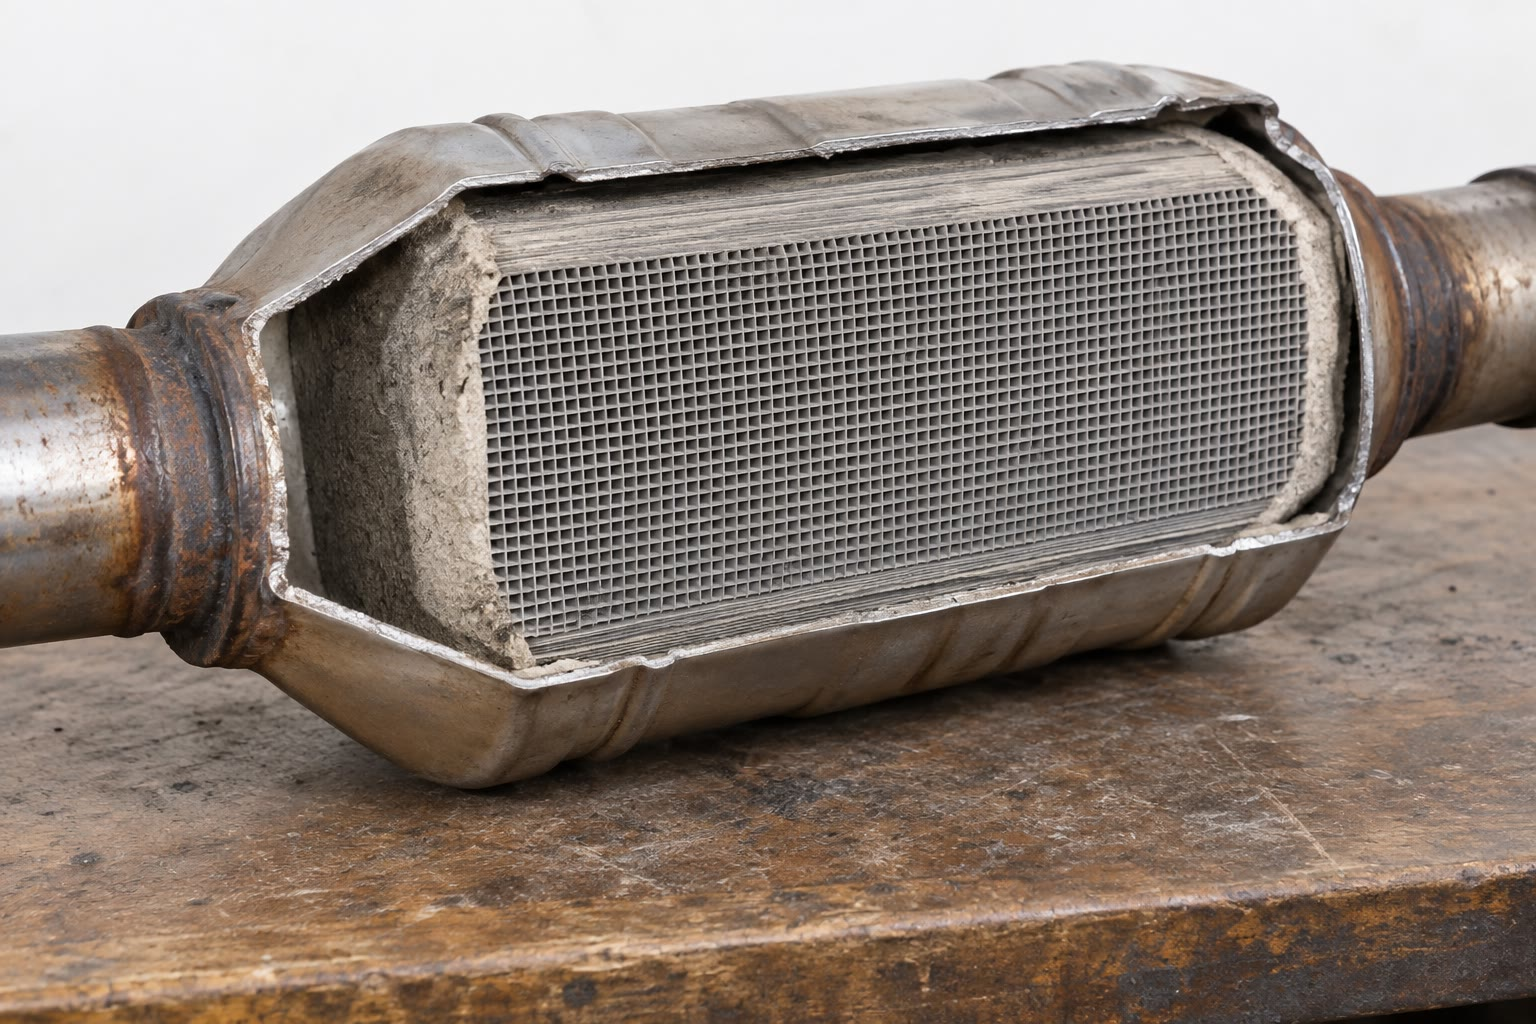
\includegraphics[width=0.45\linewidth]{images/book1/ai/g12-catalytic-converter.jpg}

{\small A catalytic converter cut open: the honeycomb core.}
\end{omfigure}

\begin{history}[Haber, Bosch and ammonia]
% ledger: haber:T, haber:p, nh3:world-2024
At the beginning of the twentieth century the chemist Fritz Haber found
how to combine the nitrogen of the \omterm{def:g4:air-a-mixture-of-gases:air}{air} with hydrogen,
\ce{N2 + 3H2 -> 2NH3}, on an iron-based \omterm{def:g12:catalysis:catalyst}{catalyst}, and the engineer Carl
Bosch turned it into an industrial process. It still runs today at 400
to \qty{500}{\celsius} and 150 to \qty{250}{atm}. In 2024 the world made
ammonia containing about 150 million tonnes of nitrogen, most of it for
fertilisers: a large share of the nitrogen in the food we eat has passed
through such a \omterm{def:g12:catalysis:catalyst}{catalyst}.
\end{history}

\section{Enzymes}

\begin{definition}[Enzyme]\label{def:g12:catalysis:enzyme}
An \emph{enzyme}\index{enzyme} is a protein made by a living organism
that catalyses one reaction of its chemistry. Enzymes are very efficient
and very specific: each fits a few \omterm{def:g7:atoms-and-molecules:molecule}{molecules} only, and they work best in
a narrow range of temperature and acidity.
\end{definition}

\begin{example}[Catalase]\label{ex:g12:catalysis:catalase}
Hydrogen peroxide is formed in cells as a by-product, and is harmful to
them. The \omterm{def:g12:catalysis:enzyme}{enzyme} catalase, present in blood, liver and many plant
tissues, decomposes it into water and oxygen at enormous speed: that is
the foam on a grazed knee, or on a slice of raw potato. Boiled potato
gives no foam: heating has destroyed the shape of the \omterm{def:g12:catalysis:enzyme}{enzyme}.
\end{example}

\begin{omfigure}
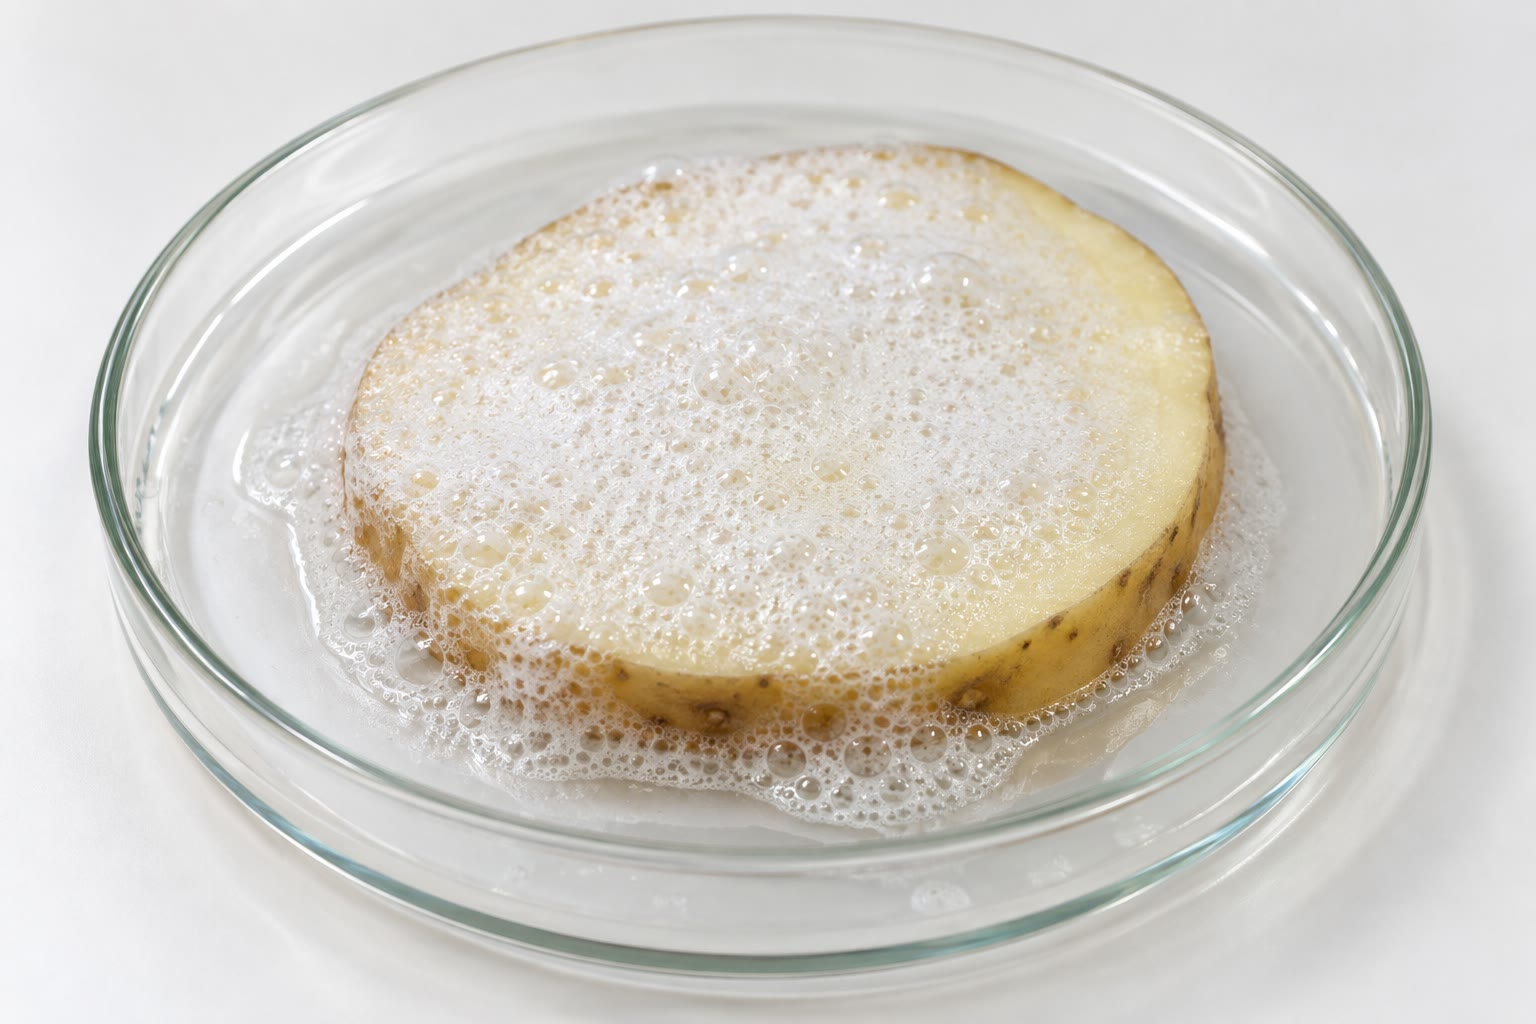
\includegraphics[width=0.45\linewidth]{images/book1/ai/g12-potato-peroxide.jpg}

{\small Hydrogen peroxide on a slice of raw potato: catalase at work.}
\end{omfigure}

\section{Selectivity}

\begin{definition}[Selective catalyst]\label{def:g12:catalysis:selective}
When the same \omterm{def:g7:chemical-reactions:reactant}{reactants} can give several reactions, a \emph{selective
catalyst}\index{selective catalyst} speeds up one of them much more than
the others, and so decides which products form.
\end{definition}

\begin{example}[Two fates of ethanol]\label{ex:g12:catalysis:ethanol}
Hot ethanol vapour passed over alumina loses water and gives ethene,
\ce{C2H5OH -> C2H4 + H2O} (an \omterm{def:g12:curly-arrows:categories}{elimination}); passed over hot copper, it
loses hydrogen and gives ethanal, \ce{C2H5OH -> CH3CHO + H2}. Same
\omterm{def:g7:chemical-reactions:reactant}{reactant}, two \omterm{def:g12:catalysis:catalyst}{catalysts}, two products.
\end{example}

\begin{remark}[Industry and life run on catalysts]\label{rem:g12:catalysis:everywhere}
Most products of the chemical industry, from \omterm{def:g4:what-a-fire-needs:fuel}{fuels} to \omterm{def:g8:plastics:plastic}{plastics} and
fertilisers, are made with \omterm{def:g12:catalysis:catalyst}{catalysts}; finding a more active or more
\omterm{def:g12:catalysis:selective}{selective catalyst} saves energy and waste. Every reaction of a living
cell is catalysed by an \omterm{def:g12:catalysis:enzyme}{enzyme}.
\end{remark}

\begin{safety}{\ghs[0.82cm]{GHS03}\ghs[0.82cm]{GHS05}\ghs[0.82cm]{GHS07}}
% ledger: ghs:H2O2
Concentrated hydrogen peroxide is a strong \omterm{def:g11:redox:oxidant}{oxidant} that can feed a fire,
burns the skin and the eyes, and is harmful if swallowed. The dilute
solutions of the laboratory still need goggles and gloves; the
decomposition releases oxygen, so it is never done in a closed vessel.
\end{safety}

\section{Exercises}


\begin{exercise}[$\star$]\label{exo:g12:catalysis:1}
In the decomposition of hydrogen peroxide catalysed by iodide \omterm{def:g9:ions:ion}{ions}, which
species are \omterm{def:g7:chemical-reactions:reactant}{reactants}, which are products, which is the \omterm{def:g12:catalysis:catalyst}{catalyst}, which
is an intermediate?
\end{exercise}

\begin{exercise}[$\star$]\label{exo:g12:catalysis:2}
Homogeneous or \omterm{def:g12:catalysis:homogeneous}{heterogeneous catalysis}: iodide \omterm{def:g9:ions:ion}{ions} in hydrogen peroxide
solution; platinum in a catalytic converter; iron in the ammonia
\omterm{def:g10:synthesis-yield:synthesis}{synthesis}; iron(III) \omterm{def:g9:ions:ion}{ions} in hydrogen peroxide solution?
\end{exercise}

\begin{exercise}[$\star$]\label{exo:g12:catalysis:3}
On the energy profiles, which path has the higher barrier? Are the
starting and final energies the same on both paths? What does this mean
for the products?
\end{exercise}

\begin{exercise}[$\star$]\label{exo:g12:catalysis:4}
Why does a \omterm{def:g12:catalysis:catalyst}{catalyst} not appear in the overall equation of a reaction?
\end{exercise}

\begin{exercise}[$\star$]\label{exo:g12:catalysis:5}
Why are the solid \omterm{def:g12:catalysis:catalyst}{catalysts} of industry used as fine powders or as thin
coats on porous supports?
\end{exercise}

\begin{exercise}[$\star\star$]\label{exo:g12:catalysis:6}
Add the two steps of the iron(III)-catalysed decomposition of hydrogen
peroxide, and show that the iron \omterm{def:g9:ions:ion}{ions} and the hydrogen \omterm{def:g9:ions:ion}{ions} cancel.
\end{exercise}

\begin{exercise}[$\star\star$]\label{exo:g12:catalysis:7}
Read the curves of the oxygen given off. How long does each run take to
release half of the final volume? By what factor does the \omterm{def:g12:catalysis:catalyst}{catalyst}
shorten it?
\end{exercise}

\begin{exercise}[$\star\star$]\label{exo:g12:catalysis:8}
Leaded petrol is not used in cars fitted with a catalytic converter: the
lead deposits on the platinum and stays there. Explain why this ruins the
converter, although the platinum is not used up by the normal reaction.
\end{exercise}

\begin{exercise}[$\star\star$]\label{exo:g12:catalysis:9}
A student measures the foam produced by potato slices in hydrogen
peroxide at 10, 25, 37, 60 and \qty{80}{\celsius}: the foam grows up to
about \qty{37}{\celsius}, then falls, and nearly vanishes at
\qty{80}{\celsius}. Explain both parts of the curve.
\end{exercise}

\begin{exercise}[$\star\star$]\label{exo:g12:catalysis:10}
Write the equation of the reaction in a catalytic converter between
carbon monoxide and nitrogen monoxide, and check that it is balanced.
Why are both pollutants removed at once?
\end{exercise}

\begin{exercise}[$\star\star$]\label{exo:g12:catalysis:11}
\qty{10.0}{mL} of hydrogen peroxide solution give off \qty{72}{mL} of
oxygen at \qty{20}{\celsius} when decomposed completely. Compute the
amount of oxygen ($V_m = \qty{24.1}{L/mol}$), then the concentration of
the solution in hydrogen peroxide.
\end{exercise}

\begin{exercise}[$\star\star\star$]\label{exo:g12:catalysis:12}
Ethanol vapour passed over alumina gives ethene; over copper it gives
ethanal. Write both equations, give the category of the first, and
explain what a \omterm{def:g12:catalysis:selective}{selective catalyst} is.
\end{exercise}

\begin{exercise}[$\star\star\star$]\label{exo:g12:catalysis:13}
A \omterm{def:g12:catalysis:catalyst}{catalyst} makes a reaction ten times faster. A student claims it also
gives ten times more product. Correct the claim, using the curves of the
oxygen given off.
\end{exercise}

\begin{exercise}[$\star\star\star$]\label{exo:g12:catalysis:14}
A \omterm{def:g7:atoms-and-molecules:molecule}{molecule} of catalase decomposes about a few million \omterm{def:g7:atoms-and-molecules:molecule}{molecules} of
hydrogen peroxide per second. Taking $\num{5e6}$ per second, how long
does one \omterm{def:g12:catalysis:enzyme}{enzyme} \omterm{def:g7:atoms-and-molecules:molecule}{molecule} take to decompose one \omterm{def:g10:the-mole:amount}{mole} of hydrogen peroxide?
How many \omterm{def:g12:catalysis:enzyme}{enzyme} \omterm{def:g7:atoms-and-molecules:molecule}{molecules} would do it in one second? (A computation on
orders of magnitude; the rate is exercise data.)
\end{exercise}

\begin{exercise}[$\star\star\star$]\label{exo:g12:catalysis:15}
% ledger: nh3:world-2024
The world made about 150 million tonnes of nitrogen in ammonia in 2024.
What mass of ammonia is that? What amount of dinitrogen was combined?
\end{exercise}

\section{Problem: The Hairdresser's Peroxide}

\begin{problem}[{Weekend problem --- what is the concentration of
``20-volume'' hydrogen peroxide?}]
\label{pb:g12:catalysis:1}
% ledger: const:Vm1, ghs:H2O2, aw:H, aw:O
Hairdressers use hydrogen peroxide solutions labelled in ``volumes'': a
``20-volume'' solution is one of which \qty{1}{L} gives off \qty{20}{L}
of oxygen when it decomposes completely, the gas being measured at
\qty{0}{\celsius} and normal atmospheric pressure, where one \omterm{def:g10:the-mole:amount}{mole} of gas
occupies \qty{22.4}{L}.

\medskip
\noindent\textbf{Part I --- The decomposition.}
\begin{enumerate}
  \item Write the equation of the decomposition of hydrogen peroxide.
  \item Is the decomposition a \omterm{def:g11:redox:reaction}{redox reaction}? Find the \omterm{def:g11:redox:oxidant}{oxidant} and the
        \omterm{def:g11:redox:oxidant}{reductant} (hydrogen peroxide is both).
  \item Why does a bottle keep for months, though the reaction is
        possible?
\end{enumerate}

\medskip
\noindent\textbf{Part II --- What ``20 volumes'' means.}
\begin{enumerate}[resume]
  \item What amount of oxygen does \qty{1}{L} of the solution give off?
  \item Deduce the amount of hydrogen peroxide in \qty{1}{L}.
  \item Give the \omterm{def:g10:concentration-and-dilution:molar-concentration}{molar concentration}.
  \item Compute the \omterm{def:g10:the-mole:molar-mass}{molar mass} of hydrogen peroxide and the \omterm{def:g10:concentration-and-dilution:mass-concentration}{mass
        concentration}.
  \item What would ``10 volumes'' mean in \omterm{def:g10:the-mole:amount}{moles} per litre?
\end{enumerate}

\medskip
\noindent\textbf{Part III --- Two \omterm{def:g12:catalysis:catalyst}{catalysts}.}
\begin{enumerate}[resume]
  \item A drop of blood (catalase) and a few drops of iron(III) chloride
        are each added to a sample. Which \omterm{def:g12:catalysis:catalyst}{catalysis} is each?
  \item Write the two steps of the iron(III) \omterm{def:g12:catalysis:catalyst}{catalysis} and check that
        their sum is the decomposition.
  \item Using the curves of the oxygen given off, describe how the volume
        of oxygen changes with and without \omterm{def:g12:catalysis:catalyst}{catalyst}, and what stays the
        same.
  \item Why does the colour of an iron(III)-catalysed sample change during
        the reaction and come back at the end?
  \item Why does a boiled potato not make the solution foam?
\end{enumerate}

\medskip
\noindent\textbf{Part IV --- The bottle.}
\begin{enumerate}[resume]
  \item What volume of oxygen, measured at \qty{0}{\celsius}, can a
        \qty{100}{mL} bottle give off?
  \item What volume is that at \qty{20}{\celsius} ($V_m =
        \qty{24.1}{L/mol}$)?
  \item Why must the cap of such a bottle let gas escape slowly?
  \item A bottle stored for a long time is titrated and found to contain
        \qty{1.50}{mol/L}. How many ``volumes'' is that now?
  \item What fraction of the hydrogen peroxide has decomposed?
  \item State the final answer: what is the \omterm{def:g10:concentration-and-dilution:molar-concentration}{molar concentration} of a
        ``20-volume'' hydrogen peroxide solution?
\end{enumerate}
\end{problem}
